Data and MC samples are compared with different Z+jets MC samples with different generators.
The following Good Run List is used with total luminosity $3.3~\text{fb}^{-1}$:
\small
\begin{verbatim}
data15_13TeV.periodAllYear_DetStatus-v73-pro19-08_DQDefects-00-01-02_PHYS_StandardGRL_All_Good_25ns.xml
\end{verbatim}
\normalsize

The following data samples are used:
\small
\begin{verbatim}
data15_13TeV.00276262.physics_Main.merge.DAOD_SUSY2.f620_m1480_p2425/
data15_13TeV.00276329.physics_Main.merge.DAOD_SUSY2.f620_m1480_p2425/
data15_13TeV.00276336.physics_Main.merge.DAOD_SUSY2.f620_m1480_p2425/
data15_13TeV.00276416.physics_Main.merge.DAOD_SUSY2.f620_m1480_p2425/
data15_13TeV.00276511.physics_Main.merge.DAOD_SUSY2.f620_m1480_p2425/
data15_13TeV.00276689.physics_Main.merge.DAOD_SUSY2.f623_m1480_p2425/
data15_13TeV.00276778.physics_Main.merge.DAOD_SUSY2.f620_m1480_p2425/
data15_13TeV.00276790.physics_Main.merge.DAOD_SUSY2.f620_m1480_p2425/
data15_13TeV.00276952.physics_Main.merge.DAOD_SUSY2.f620_m1480_p2425/
data15_13TeV.00276954.physics_Main.merge.DAOD_SUSY2.f620_m1480_p2425/
data15_13TeV.00278880.physics_Main.merge.DAOD_SUSY2.f628_m1497_p2425/
data15_13TeV.00278912.physics_Main.merge.DAOD_SUSY2.f628_m1497_p2425/
data15_13TeV.00278968.physics_Main.merge.DAOD_SUSY2.f628_m1497_p2425/
data15_13TeV.00279169.physics_Main.merge.DAOD_SUSY2.f628_m1497_p2425/
data15_13TeV.00279259.physics_Main.merge.DAOD_SUSY2.f628_m1497_p2425/
data15_13TeV.00279279.physics_Main.merge.DAOD_SUSY2.f628_m1497_p2425/
data15_13TeV.00279284.physics_Main.merge.DAOD_SUSY2.f628_m1497_p2425/
data15_13TeV.00279345.physics_Main.merge.DAOD_SUSY2.f628_m1497_p2425/
data15_13TeV.00279515.physics_Main.merge.DAOD_SUSY2.f628_m1497_p2425/
data15_13TeV.00279598.physics_Main.merge.DAOD_SUSY2.f628_m1497_p2425/
data15_13TeV.00279685.physics_Main.merge.DAOD_SUSY2.f628_m1497_p2425/
data15_13TeV.00279764.physics_Main.merge.DAOD_SUSY2.f628_m1497_p2425/
data15_13TeV.00279813.physics_Main.merge.DAOD_SUSY2.f628_m1497_p2425/
data15_13TeV.00279867.physics_Main.merge.DAOD_SUSY2.f628_m1497_p2425/
data15_13TeV.00279928.physics_Main.merge.DAOD_SUSY2.f628_m1497_p2425/
data15_13TeV.00279932.physics_Main.merge.DAOD_SUSY2.f629_m1504_p2425/
data15_13TeV.00279984.physics_Main.merge.DAOD_SUSY2.f629_m1504_p2425/
data15_13TeV.00280231.physics_Main.merge.DAOD_SUSY2.f630_m1504_p2425/
data15_13TeV.00280319.physics_Main.merge.DAOD_SUSY2.f629_m1504_p2425/
data15_13TeV.00280368.physics_Main.merge.DAOD_SUSY2.f629_m1504_p2436/
data15_13TeV.00280423.physics_Main.merge.DAOD_SUSY2.f629_m1504_p2425/
data15_13TeV.00280464.physics_Main.merge.DAOD_SUSY2.f629_m1504_p2425/
data15_13TeV.00280500.physics_Main.merge.DAOD_SUSY2.f631_m1504_p2425/
data15_13TeV.00280520.physics_Main.merge.DAOD_SUSY2.f632_m1504_p2425/
data15_13TeV.00280614.physics_Main.merge.DAOD_SUSY2.f629_m1504_p2425/
data15_13TeV.00280673.physics_Main.merge.DAOD_SUSY2.f629_m1504_p2425/
data15_13TeV.00280753.physics_Main.merge.DAOD_SUSY2.f629_m1504_p2425/
data15_13TeV.00280853.physics_Main.merge.DAOD_SUSY2.f629_m1504_p2425/
data15_13TeV.00280862.physics_Main.merge.DAOD_SUSY2.f629_m1504_p2425/
data15_13TeV.00280950.physics_Main.merge.DAOD_SUSY2.f629_m1504_p2425/
data15_13TeV.00280977.physics_Main.merge.DAOD_SUSY2.f629_m1504_p2425/
data15_13TeV.00281070.physics_Main.merge.DAOD_SUSY2.f629_m1504_p2425/
data15_13TeV.00281074.physics_Main.merge.DAOD_SUSY2.f629_m1504_p2425/
data15_13TeV.00281075.physics_Main.merge.DAOD_SUSY2.f629_m1504_p2425/
data15_13TeV.00281317.physics_Main.merge.DAOD_SUSY2.f629_m1504_p2425/
data15_13TeV.00281385.physics_Main.merge.DAOD_SUSY2.f629_m1504_p2425/
data15_13TeV.00281411.physics_Main.merge.DAOD_SUSY2.f629_m1504_p2425/
data15_13TeV.00282625.physics_Main.merge.DAOD_SUSY2.f640_m1511_p2425/
data15_13TeV.00282631.physics_Main.merge.DAOD_SUSY2.f640_m1511_p2425/
data15_13TeV.00282712.physics_Main.merge.DAOD_SUSY2.f640_m1511_p2425/
data15_13TeV.00282784.physics_Main.merge.DAOD_SUSY2.f640_m1511_p2425/
data15_13TeV.00282992.physics_Main.merge.DAOD_SUSY2.f640_m1511_p2425/
data15_13TeV.00283074.physics_Main.merge.DAOD_SUSY2.f640_m1511_p2425/
data15_13TeV.00283155.physics_Main.merge.DAOD_SUSY2.f640_m1511_p2425/
data15_13TeV.00283270.physics_Main.merge.DAOD_SUSY2.f640_m1511_p2425/
data15_13TeV.00283429.physics_Main.merge.DAOD_SUSY2.f643_m1518_p2425/
data15_13TeV.00283608.physics_Main.merge.DAOD_SUSY2.f643_m1518_p2425/
data15_13TeV.00283780.physics_Main.merge.DAOD_SUSY2.f643_m1518_p2425/
data15_13TeV.00284006.physics_Main.merge.DAOD_SUSY2.f643_m1518_p2425/
data15_13TeV.00284154.physics_Main.merge.DAOD_SUSY2.f643_m1518_p2425/
data15_13TeV.00284213.physics_Main.merge.DAOD_SUSY2.f643_m1518_p2425/
data15_13TeV.00284285.physics_Main.merge.DAOD_SUSY2.f643_m1518_p2425/
data15_13TeV.00284420.physics_Main.merge.DAOD_SUSY2.f643_m1518_p2425/
data15_13TeV.00284427.physics_Main.merge.DAOD_SUSY2.f643_m1518_p2425/
data15_13TeV.00284484.physics_Main.merge.DAOD_SUSY2.f644_m1518_p2425/
\end{verbatim}
\normalsize

Z+jets samples generated by Powheg and MadGraph are compared, while other background MC samples are generated by Powheg.
The following MC samples are used for other background including $t\bar{t}$ and single top:
\scriptsize
\begin{verbatim}
mc15_13TeV.410000.PowhegPythiaEvtGen_P2012_ttbar_hdamp172p5_nonallhad.merge.DAOD_SUSY2.e3698_s2608_s2183_r6765_r6282_p2419/
mc15_13TeV.410015.PowhegPythiaEvtGen_P2012_Wt_dilepton_top.merge.DAOD_SUSY2.e3753_s2608_s2183_r6869_r6282_p2419/
mc15_13TeV.410016.PowhegPythiaEvtGen_P2012_Wt_dilepton_antitop.merge.DAOD_SUSY2.e3753_s2608_s2183_r6869_r6282_p2419/
\end{verbatim}
\normalsize

A signal MC sample is used for reference.
The following signal MC sample is used:
\scriptsize
\begin{verbatim}
mc15_13TeV.392200.MGPy8EG_A14N23LO_C1N2_WZ_350p0_250p0_3L_2L7.merge.DAOD_SUSY2.e4287_a766_a777_r6282_p2419/
\end{verbatim}
\normalsize

\subsection{pileup reweighting}
In this section, all background samples are reweighted according to pileup reweighting.
\subsubsection{Powheg samples}
The following Z+jets samples with Powheg generator are used:
\scriptsize
\begin{verbatim}
mc15_13TeV.361106.PowhegPythia8EvtGen_AZNLOCTEQ6L1_Zee.merge.DAOD_SUSY2.e3601_s2576_s2132_r6765_r6282_p2419/
mc15_13TeV.361107.PowhegPythia8EvtGen_AZNLOCTEQ6L1_Zmumu.merge.DAOD_SUSY2.e3601_s2576_s2132_r6765_r6282_p2419/
mc15_13TeV.361108.PowhegPythia8EvtGen_AZNLOCTEQ6L1_Ztautau.merge.DAOD_SUSY2.e3601_s2576_s2132_r6765_r6282_p2419/
\end{verbatim}
\normalsize

The comparisons for different variables are shown in Fig.~\ref{pileup_powheg_start}~-~\ref{pileup_powheg_end}.

There are great discrepancies between data and MC for mT2 variable.
The Powheg generator may not simulate the $\text{p}_{\text{T}}$ of Z very well, and the Z $\text{p}_{\text{T}}$ reweighting is done on the Z+jets samples in section~\ref{sec_zpt}.

\begin{figure}
\includegraphics[width=0.5\textwidth]{CR/pileup_powheg/pt1_ee_OS}
\includegraphics[width=0.5\textwidth]{CR/pileup_powheg/pt1_mumu_OS}
\caption{$\text{p}_{\text{T}}$ of the leading lepton for ee channel (left) and $\mu\mu$ channel (right).}
\label{pileup_powheg_start}
\end{figure}

\begin{figure}
\includegraphics[width=0.5\textwidth]{CR/pileup_powheg/pt2_ee_OS}
\includegraphics[width=0.5\textwidth]{CR/pileup_powheg/pt2_mumu_OS}
\caption{$\text{p}_{\text{T}}$ of the subleading lepton for ee channel (left) and $\mu\mu$ channel (right).}
\end{figure}

\begin{figure}
\includegraphics[width=0.5\textwidth]{CR/pileup_powheg/mll_ee_OS}
\includegraphics[width=0.5\textwidth]{CR/pileup_powheg/mll_mumu_OS}
\caption{Dilepton invariant mass for ee channel (left) and $\mu\mu$ channel (right).}
\end{figure}

\begin{figure}
\includegraphics[width=0.5\textwidth]{CR/pileup_powheg/ptll_ee_OS}
\includegraphics[width=0.5\textwidth]{CR/pileup_powheg/ptll_mumu_OS}
\caption{Dilepton $\text{p}_{\text{T}}$ for ee channel (left) and $\mu\mu$ channel (right).}
\end{figure}

\begin{figure}
\includegraphics[width=0.5\textwidth]{CR/pileup_powheg/MET_ee_OS}
\includegraphics[width=0.5\textwidth]{CR/pileup_powheg/MET_mumu_OS}
\caption{MET for ee channel (left) and $\mu\mu$ channel (right).}
\end{figure}

\begin{figure}
\includegraphics[width=0.5\textwidth]{CR/pileup_powheg/mT2_ee_OS}
\includegraphics[width=0.5\textwidth]{CR/pileup_powheg/mT2_mumu_OS}
\caption{mT2 for ee channel (left) and $\mu\mu$ channel (right).}
\end{figure}

\begin{figure}
\includegraphics[width=0.5\textwidth]{CR/pileup_powheg/nJet_ee_OS}
\includegraphics[width=0.5\textwidth]{CR/pileup_powheg/nJet_mumu_OS}
\caption{Number of jets for ee channel (left) and $\mu\mu$ channel (right).}
\end{figure}

\begin{figure}
\includegraphics[width=0.5\textwidth]{CR/pileup_powheg/nBJet_ee_OS}
\includegraphics[width=0.5\textwidth]{CR/pileup_powheg/nBJet_mumu_OS}
\caption{Number of b-jets for ee channel (left) and $\mu\mu$ channel (right).}
\label{pileup_powheg_end}
\end{figure}

\subsubsection{MadGraph samples}
The following Z+jets samples with MadGraph generator are used:
\scriptsize
\begin{verbatim}
mc15_13TeV.361500.MadGraphPythia8EvtGen_A14NNPDF23LO_Zee_Np0.merge.DAOD_SUSY2.e3898_s2608_s2183_r6869_r6282_p2419/
mc15_13TeV.361501.MadGraphPythia8EvtGen_A14NNPDF23LO_Zee_Np1.merge.DAOD_SUSY2.e3898_s2608_s2183_r6869_r6282_p2419/
mc15_13TeV.361502.MadGraphPythia8EvtGen_A14NNPDF23LO_Zee_Np2.merge.DAOD_SUSY2.e3898_s2608_s2183_r6869_r6282_p2419/
mc15_13TeV.361503.MadGraphPythia8EvtGen_A14NNPDF23LO_Zee_Np3.merge.DAOD_SUSY2.e3898_s2608_s2183_r6869_r6282_p2419/
mc15_13TeV.361504.MadGraphPythia8EvtGen_A14NNPDF23LO_Zee_Np4.merge.DAOD_SUSY2.e3898_s2608_s2183_r6869_r6282_p2419/
mc15_13TeV.361505.MadGraphPythia8EvtGen_A14NNPDF23LO_Zmumu_Np0.merge.DAOD_SUSY2.e3898_s2608_s2183_r6869_r6282_p2419/
mc15_13TeV.361506.MadGraphPythia8EvtGen_A14NNPDF23LO_Zmumu_Np1.merge.DAOD_SUSY2.e3898_s2608_s2183_r6869_r6282_p2419/
mc15_13TeV.361507.MadGraphPythia8EvtGen_A14NNPDF23LO_Zmumu_Np2.merge.DAOD_SUSY2.e3898_s2608_s2183_r6869_r6282_p2419/
mc15_13TeV.361508.MadGraphPythia8EvtGen_A14NNPDF23LO_Zmumu_Np3.merge.DAOD_SUSY2.e3898_s2608_s2183_r6869_r6282_p2419/
mc15_13TeV.361509.MadGraphPythia8EvtGen_A14NNPDF23LO_Zmumu_Np4.merge.DAOD_SUSY2.e3898_s2608_s2183_r6869_r6282_p2419/
mc15_13TeV.361510.MadGraphPythia8EvtGen_A14NNPDF23LO_Ztautau_Np0.merge.DAOD_SUSY2.e3898_s2608_s2183_r6869_r6282_p2419/
mc15_13TeV.361511.MadGraphPythia8EvtGen_A14NNPDF23LO_Ztautau_Np1.merge.DAOD_SUSY2.e3898_s2608_s2183_r6869_r6282_p2419/
mc15_13TeV.361512.MadGraphPythia8EvtGen_A14NNPDF23LO_Ztautau_Np2.merge.DAOD_SUSY2.e3898_s2608_s2183_r6869_r6282_p2419/
mc15_13TeV.361513.MadGraphPythia8EvtGen_A14NNPDF23LO_Ztautau_Np3.merge.DAOD_SUSY2.e3898_s2608_s2183_r6869_r6282_p2419/
mc15_13TeV.361514.MadGraphPythia8EvtGen_A14NNPDF23LO_Ztautau_Np4.merge.DAOD_SUSY2.e3898_s2608_s2183_r6869_r6282_p2419/
\end{verbatim}
\normalsize

The comparisons for different variables are shown in Fig.~\ref{pileup_MadGraph_start}~-~\ref{pileup_MadGraph_end}.

\begin{figure}
\includegraphics[width=0.5\textwidth]{CR/pileup_MadGraph/pt1_ee_OS}
\includegraphics[width=0.5\textwidth]{CR/pileup_MadGraph/pt1_mumu_OS}
\caption{$\text{p}_{\text{T}}$ of the leading lepton for ee channel (left) and $\mu\mu$ channel (right).}
\label{pileup_MadGraph_start}
\end{figure}

\begin{figure}
\includegraphics[width=0.5\textwidth]{CR/pileup_MadGraph/pt2_ee_OS}
\includegraphics[width=0.5\textwidth]{CR/pileup_MadGraph/pt2_mumu_OS}
\caption{$\text{p}_{\text{T}}$ of the subleading lepton for ee channel (left) and $\mu\mu$ channel (right).}
\end{figure}

\begin{figure}
\includegraphics[width=0.5\textwidth]{CR/pileup_MadGraph/mll_ee_OS}
\includegraphics[width=0.5\textwidth]{CR/pileup_MadGraph/mll_mumu_OS}
\caption{Dilepton invariant mass for ee channel (left) and $\mu\mu$ channel (right).}
\end{figure}

\begin{figure}
\includegraphics[width=0.5\textwidth]{CR/pileup_MadGraph/ptll_ee_OS}
\includegraphics[width=0.5\textwidth]{CR/pileup_MadGraph/ptll_mumu_OS}
\caption{Dilepton $\text{p}_{\text{T}}$ for ee channel (left) and $\mu\mu$ channel (right).}
\end{figure}

\begin{figure}
\includegraphics[width=0.5\textwidth]{CR/pileup_MadGraph/MET_ee_OS}
\includegraphics[width=0.5\textwidth]{CR/pileup_MadGraph/MET_mumu_OS}
\caption{MET for ee channel (left) and $\mu\mu$ channel (right).}
\end{figure}

\begin{figure}
\includegraphics[width=0.5\textwidth]{CR/pileup_MadGraph/mT2_ee_OS}
\includegraphics[width=0.5\textwidth]{CR/pileup_MadGraph/mT2_mumu_OS}
\caption{mT2 for ee channel (left) and $\mu\mu$ channel (right).}
\end{figure}

\begin{figure}
\includegraphics[width=0.5\textwidth]{CR/pileup_MadGraph/nJet_ee_OS}
\includegraphics[width=0.5\textwidth]{CR/pileup_MadGraph/nJet_mumu_OS}
\caption{Number of jets for ee channel (left) and $\mu\mu$ channel (right).}
\end{figure}

\begin{figure}
\includegraphics[width=0.5\textwidth]{CR/pileup_MadGraph/nBJet_ee_OS}
\includegraphics[width=0.5\textwidth]{CR/pileup_MadGraph/nBJet_mumu_OS}
\caption{Number of b-jets for ee channel (left) and $\mu\mu$ channel (right).}
\label{pileup_MadGraph_end}
\end{figure}

\clearpage
\subsection{Z $\text{p}_{\text{T}}$ reweighting}
\label{sec_zpt}
In this section, the Z $\text{p}_{\text{T}}$ reweighting, in addition to the pileup reweighting, is done on the Z+jets samples generated by Powheg.
The ratio of the number of Z+jets events from data to that from Z+jets MC is calculated by
\begin{equation}
\text{Ratio} = \frac{\text{(Data)}-\text{(MC of non Z+jets)}}{\text{(MC of Z+jets)}}
\end{equation}
Two different methods of fitting are used: simple fit and combined fit.

\subsubsection{Simple fit}
For the simple fit, the ratio plots are fitted by second order polynomials $y = a_0 + a_1 x + a_2 x^2$ independently.
The plots of the ratio against dilepton $\text{p}_{\text{T}}$ for ee and $\mu\mu$ channel are shown in Fig.~\ref{zpt_powheg_simple}.
\begin{figure}
\centering
\includegraphics[width=0.5\textwidth]{CR/Zpt_powheg_simple/ptll_rw}
\caption{The plots of ratio against dilepton $\text{p}_{\text{T}}$ for ee channel (black) and $\mu\mu$ channel (red).}
\label{zpt_powheg_simple}
\end{figure}
For ee channel, the fitting results are
\begin{equation}
a_0 = 0.968 \pm 0.003 \qquad
a_1 = (3.2 \pm 1.8) \times 10^{-4} \qquad
a_2 = (7.1 \pm 1.6) \times 10^{-6}
\end{equation}
For $\mu\mu$ channel, the fitting results are
\begin{equation}
a_0 = 0.940 \pm 0.002 \qquad
a_1 = (7.9 \pm 1.5) \times 10^{-4} \qquad
a_2 = (3.3 \pm 1.3) \times 10^{-6}
\end{equation}
The dilepton $\text{p}_{\text{T}}$ and mT2 are then reweighted according to the corresponding channel and their dilepton $\text{p}_{\text{T}}$.
The reweighted plots for dilepton $\text{p}_{\text{T}}$ and mT2 are shown in Fig.~\ref{zpt_powheg_simple_start}~-~\ref{zpt_powheg_simple_end}.

\begin{figure}
\includegraphics[width=0.5\textwidth]{CR/Zpt_powheg_simple/ptll_ee_OS}
\includegraphics[width=0.5\textwidth]{CR/Zpt_powheg_simple/ptll_mumu_OS}
\caption{Dilepton $\text{p}_{\text{T}}$ for ee channel (left) and $\mu\mu$ channel (right).}
\label{zpt_powheg_simple_start}
\end{figure}

\begin{figure}
\includegraphics[width=0.5\textwidth]{CR/Zpt_powheg_simple/mT2_ee_OS}
\includegraphics[width=0.5\textwidth]{CR/Zpt_powheg_simple/mT2_mumu_OS}
\caption{mT2 for ee channel (left) and $\mu\mu$ channel (right).}
\label{zpt_powheg_simple_end}
\end{figure}

\subsubsection{Combined fit}
For the combined fit, the ratio plot for the $\mu\mu$ channel is fitted by a second order polynomial $y = a_0 + a_1 x + a_2 x^2$, while the ratio plot for the ee channel is fitted by another second order polynomial with one more scale factor $c$, $y = c(a_0 + a_1 x + a_2 x^2)$.
The plots of the ratio against dilepton $\text{p}_{\text{T}}$ for ee and $\mu\mu$ channel are shown in Fig.~\ref{zpt_powheg_combined}.
\begin{figure}
\centering
\includegraphics[width=0.5\textwidth]{CR/Zpt_powheg_combined/ptll_rw}
\caption{The plots of ratio against dilepton $\text{p}_{\text{T}}$ for ee channel (black) and $\mu\mu$ channel (red).}
\label{zpt_powheg_combined}
\end{figure}
The fitting results are
\begin{equation}
a_0 = 0.942 \pm 0.002 \qquad
a_1 = (5.9 \pm 1.1) \times 10^{-4} \qquad
a_2 = (4.8 \pm 1.0) \times 10^{-6} \qquad
c =  1.023 \pm 0.002
\end{equation}
The dilepton $\text{p}_{\text{T}}$ and mT2 are then reweighted according to the fitting function of the $\mu\mu$ channel and their dilepton $\text{p}_{\text{T}}$.
The reweighted plots for dilepton $\text{p}_{\text{T}}$ and mT2 are shown in Fig.~\ref{zpt_powheg_combined_start}~-~\ref{zpt_powheg_combined_end}.

\begin{figure}
\includegraphics[width=0.5\textwidth]{CR/Zpt_powheg_combined/ptll_ee_OS}
\includegraphics[width=0.5\textwidth]{CR/Zpt_powheg_combined/ptll_mumu_OS}
\caption{Dilepton $\text{p}_{\text{T}}$ for ee channel (left) and $\mu\mu$ channel (right).}
\label{zpt_powheg_combined_start}
\end{figure}

\begin{figure}
\includegraphics[width=0.5\textwidth]{CR/Zpt_powheg_combined/mT2_ee_OS}
\includegraphics[width=0.5\textwidth]{CR/Zpt_powheg_combined/mT2_mumu_OS}
\caption{mT2 for ee channel (left) and $\mu\mu$ channel (right).}
\label{zpt_powheg_combined_end}
\end{figure}
